\clearpage
\section{新星景モード（星も地上もくっきり）}\label{sec:nightscape}

\subsection{しくみ}

星は時間とともに動き、地上は動きません（追尾撮影では反対に、星が止まって地上が動きます）。
そのため、星に合わせて重ねると地上がにじみ、地上に合わせて重ねると星がにじみます。

新星景モードでは、\textbf{空は星に合わせて}、\textbf{地上は地上に合わせて}それぞれ重ね、空と地上の境目でつなぎ合わせます。
空と地上の境目は、写真を見比べて自動で見つけます。違っている所は、ブラシで塗って直せます。

\begin{center}
\begin{tikzpicture}[font=\sffamily\small,
  box/.style={draw=black!40,rounded corners=3pt,minimum width=3.2cm,minimum height=1.0cm,align=center},
  arr/.style={-{Stealth[length=2.4mm]},accentdark,line width=1pt}]
  \node[box,fill=skyblue!12] (sky) at (0,0.8) {空は\textbf{星}に合わせて重ねる};
  \node[box,fill=groundgreen!12] (ground) at (0,-0.8) {地上は\textbf{地上}に合わせて重ねる};
  \node[box,fill=accent!12,minimum width=3.6cm] (mix) at (5.2,0) {境目でつなぐ\\（自動で判定＋ブラシで直す）};
  \node[box,fill=black!5,minimum width=2.4cm] (out) at (9.4,0) {星も地上も\\くっきりした1枚};
  \draw[arr] (sky.east) -- (mix.west); \draw[arr] (ground.east) -- (mix.west); \draw[arr] (mix) -- (out);
\end{tikzpicture}
\end{center}

\begin{memo}
新星景モードは、スタック方式が\ui{平均}か\ui{中央値}のときに使えます（中央値を選んだ場合も、外れ値を除いた平均で合成します）。
動く星や飛行機の光を除くために、シグマクリッピングの κ の設定を使います。
\end{memo}

\subsection{使い方の流れ}

\begin{center}
\begin{tikzpicture}[node distance=0.32cm,
  box/.style={draw=accentdark,fill=accent!12,rounded corners=3pt,minimum height=1.1cm,text width=2.3cm,
    align=center,font=\sffamily\small},
  arr/.style={-{Stealth[length=2.4mm]},accentdark,line width=1pt}]
  \node[box] (a) {\textbf{1} 新星景モードを\\ON にする};
  \node[box,right=of a] (b) {\textbf{2}\ui{解析開始}\\を押す};
  \node[box,right=of b] (c) {\textbf{3} 違う所を\\ブラシで直す};
  \node[box,right=of c] (d) {\textbf{4} スタッキング\\開始};
  \node[box,right=of d] (e) {\textbf{5} 結果を見て\\必要なら塗り直す};
  \draw[arr] (a) -- (b); \draw[arr] (b) -- (c); \draw[arr] (c) -- (d); \draw[arr] (d) -- (e);
  \draw[arr] (e.south) -- ++(0,-0.45) -| (c.south);
\end{tikzpicture}
\end{center}

\subsubsection*{手順1　新星景モードを ON にする}

Light の写真を読み込み、スタック方式を\ui{平均}にしてから、\ui{空と地上（新星景モード）}の欄の\ui{新星景モード}にチェックを入れます。

\begin{figure}[H]
\centering
\begin{screenshot}[0.5\linewidth]{settings_nightscape}
  \calloutleft{1}{check}
  \calloutleft{2}{register}
  \calloutleft{3}{analyze}
  \calloutleft{4}{brush}
  \calloutleft{5}{size}
  \calloutleft{6}{feather}
  \calloutleft{7}{clearmask}
\end{screenshot}
\caption{\ui{空と地上（新星景モード）}の欄}
\end{figure}

\begin{callouts}
\co{1} \ui{新星景モード}：チェックを入れると、空と地上を分けて合成します。その下に、いまの状態や次にすることが表示されます。
\co{2} \ui{地上固定フレーム登録…}：地上だけを撮った写真を登録します（\ref{sec:groundfixed}節）。\ui{解除}で外します。
\co{3} \ui{解析開始}：全部の写真を調べて、空と地上を自動で塗り分けます。
\co{4} \textbf{ブラシの種類}：\ui{空（青）}・\ui{地上（緑）}・\ui{消しゴム}を選びます。
\co{5} \textbf{ブラシの大きさ}（5〜150 px）。
\co{6} \textbf{境界ぼかし}（0〜300 px、最初は 0 px）：空と地上の境目をさらになじませます（\ref{sec:feather}節）。
\co{7} \ui{マスクをクリア}：塗った色（自動の判定も含む）をすべて消します（\key{⌘}\,\key{K}）。
\end{callouts}

\subsubsection*{手順2　\ui{解析開始}を押す}

\ui{解析開始}を押すと、全部の写真の位置を星と地上のそれぞれで合わせ、空と地上を自動で判定します。
写真の枚数や Mac によって、数分かかります（ボタンに進み具合が表示されます）。

終わると、基準画像の上に、空が\textcolor{skyblue}{\textbf{青}}、地上が\textcolor{groundgreen}{\textbf{緑}}で半透明に塗られます。

\begin{figure}[H]
\centering
\begin{screenshot}{main_analyzed}
  \calloutat{1}{0.40}{0.70}{90}{0.9}
  \calloutat{2}{0.45}{0.28}{-90}{0.9}
  \calloutright{3}{status}
\end{screenshot}
\caption{解析が終わったところ。\num{1}空（青）と\num{2}地上（緑）に塗り分けられ、\num{3}に結果が表示されます}
\end{figure}

\begin{memo}[境目は塗られていません]
空と地上の境目のすぐ近くは、わざと塗らずに残してあります。境目は、合成するときに写真の輪郭に沿って自動で決めます。
\end{memo}

\subsubsection*{手順3　違う所をブラシで直す}

自動の判定が違っている所があれば、ブラシで塗り直します。
\begin{steps}
  \item \ui{空（青）}か\ui{地上（緑）}を選びます。
  \item プレビューの上でドラッグして塗ります。塗った所は、自動の判定より優先されます。
  \item 塗りすぎた所は\ui{消しゴム}で消すと、自動の判定に戻ります。
\end{steps}

\begin{figure}[H]
\centering
\begin{minipage}[t]{0.49\linewidth}\centering
\begin{screenshot}{canvas_analyzed}
  \circleat{0.07}{0.44}{1.0}
\end{screenshot}\\[0.3ex]{\small 直す前：左端の空の一部が地上（緑）になっている（左下を拡大）}
\end{minipage}\hfill
\begin{minipage}[t]{0.49\linewidth}\centering
\begin{screenshot}{canvas_brushed}
  \circleat{0.07}{0.44}{1.0}
\end{screenshot}\\[0.3ex]{\small 直した後：空（青）のブラシで塗った}
\end{minipage}
\caption{ブラシで直す例}
\end{figure}

\begin{hint}[ブラシのこつ]
\begin{itemize}[itemsep=0.2ex,leftmargin=1.2em]
  \item 境目ぴったりに塗る必要はありません。少しはみ出して塗っても、はみ出した所は写真の輪郭に合わせて自動で直ります。
  \item 細かい所は、写真を拡大してから（ピンチ、または\key{⌘}＋スクロール）小さなブラシで塗ります。
  \item 拡大した写真を動かすときは、\key{space}キーか\key{option}キーを押しながらドラッグします。
\end{itemize}
\end{hint}

\subsubsection*{手順4　スタッキング開始}

\ui{★ スタッキング開始}を押します。手順2の解析の結果を使うので、位置合わせはやり直しません。

\begin{figure}[H]
\centering
\begin{screenshot}{main_result}
  \calloutabove{1}{toggle}
  \calloutright{2}{status}
\end{screenshot}
\caption{新星景モードで合成したところ}
\end{figure}

\begin{callouts}
\co{1} \ui{元画像を表示}：押すと元の写真とマスクの表示に戻り、ブラシで塗り直せます。
\co{2} 「新星景モード・…で合成」と表示されれば、空と地上を分けて合成できています。
\end{callouts}

\subsubsection*{手順5　結果を見て、必要なら塗り直す}

結果を拡大して、空と地上の境目を確かめます。気になる所があれば、\ui{元画像を表示}を押してブラシで塗り直し、もう一度\ui{★ スタッキング開始}を押します。
2回目からは解析をやり直さないので、早く終わります。

\begin{caution}[解析をやり直すとき]
Light の写真・基準画像・Dark などを変えたときは、前の解析の結果は使えません。もう一度\ui{解析開始}を押してください（ブラシで塗った所は残ります）。
\end{caution}

\subsection{地上固定フレーム}\label{sec:groundfixed}

星を追尾して撮ると、地上は写真ごとに流れてしまいます。そのようなとき、追尾を止めて地上だけを撮った写真（\textbf{地上固定フレーム}）があれば、地上はその写真を使い、その構図で合成できます。

\begin{steps}
  \item 新星景モードをONにして、\ui{地上固定フレーム登録…}を押し、地上を撮った写真を選びます（何枚でも）。
  \item ファイルリストの Light タブのいちばん上に\ui{地上固定フレーム}の欄ができ、登録した写真が並びます。
  \item \ui{解析開始}を押します。今度は地上固定フレームの上に、空と地上が塗り分けられます。
  \item あとはふつうの新星景モードと同じです（ブラシで直して、スタッキング開始）。
\end{steps}

\begin{figure}[H]
\centering
\begin{screenshot}{main_groundfixed}
  \calloutleft{1}{section}
  \calloutright{2}{register}
\end{screenshot}
\caption{地上固定フレームを登録して解析したところ。\num{1}登録した写真、\num{2}登録のボタン（枚数が表示されます）}
\end{figure}

\begin{itemize}[itemsep=0.4ex]
  \item \textbf{撮り方}：Light と同じ三脚・同じ位置で、追尾撮影の\textbf{直前か直後}に続けて撮ってください。前と後の両方の写真を混ぜると、地上が二重になります（写真どうしの位置合わせはしません）。
  \item \textbf{複数枚}：画素ごとの中央値で1枚にまとめます（2枚なら平均）。露出の違う写真（AEB など）でもかまいません。撮影情報（露出時間・ISO・F値）から、明るさを Light に揃えます。白飛びした所は使いません。
  \item \textbf{補正}：Dark は露出時間が違うので、地上固定フレームには使いません（Flat・Bias は使います）。
  \item \textbf{RAW}：Light が RAW のときは、同じカメラの RAW を登録してください。
  \item \textbf{マスク}：登録したり外したりすると、マスクの構図が変わるので、塗ったマスクは消えます。もう一度\ui{解析開始}を押してください。
\end{itemize}

\begin{figure}[H]
\centering
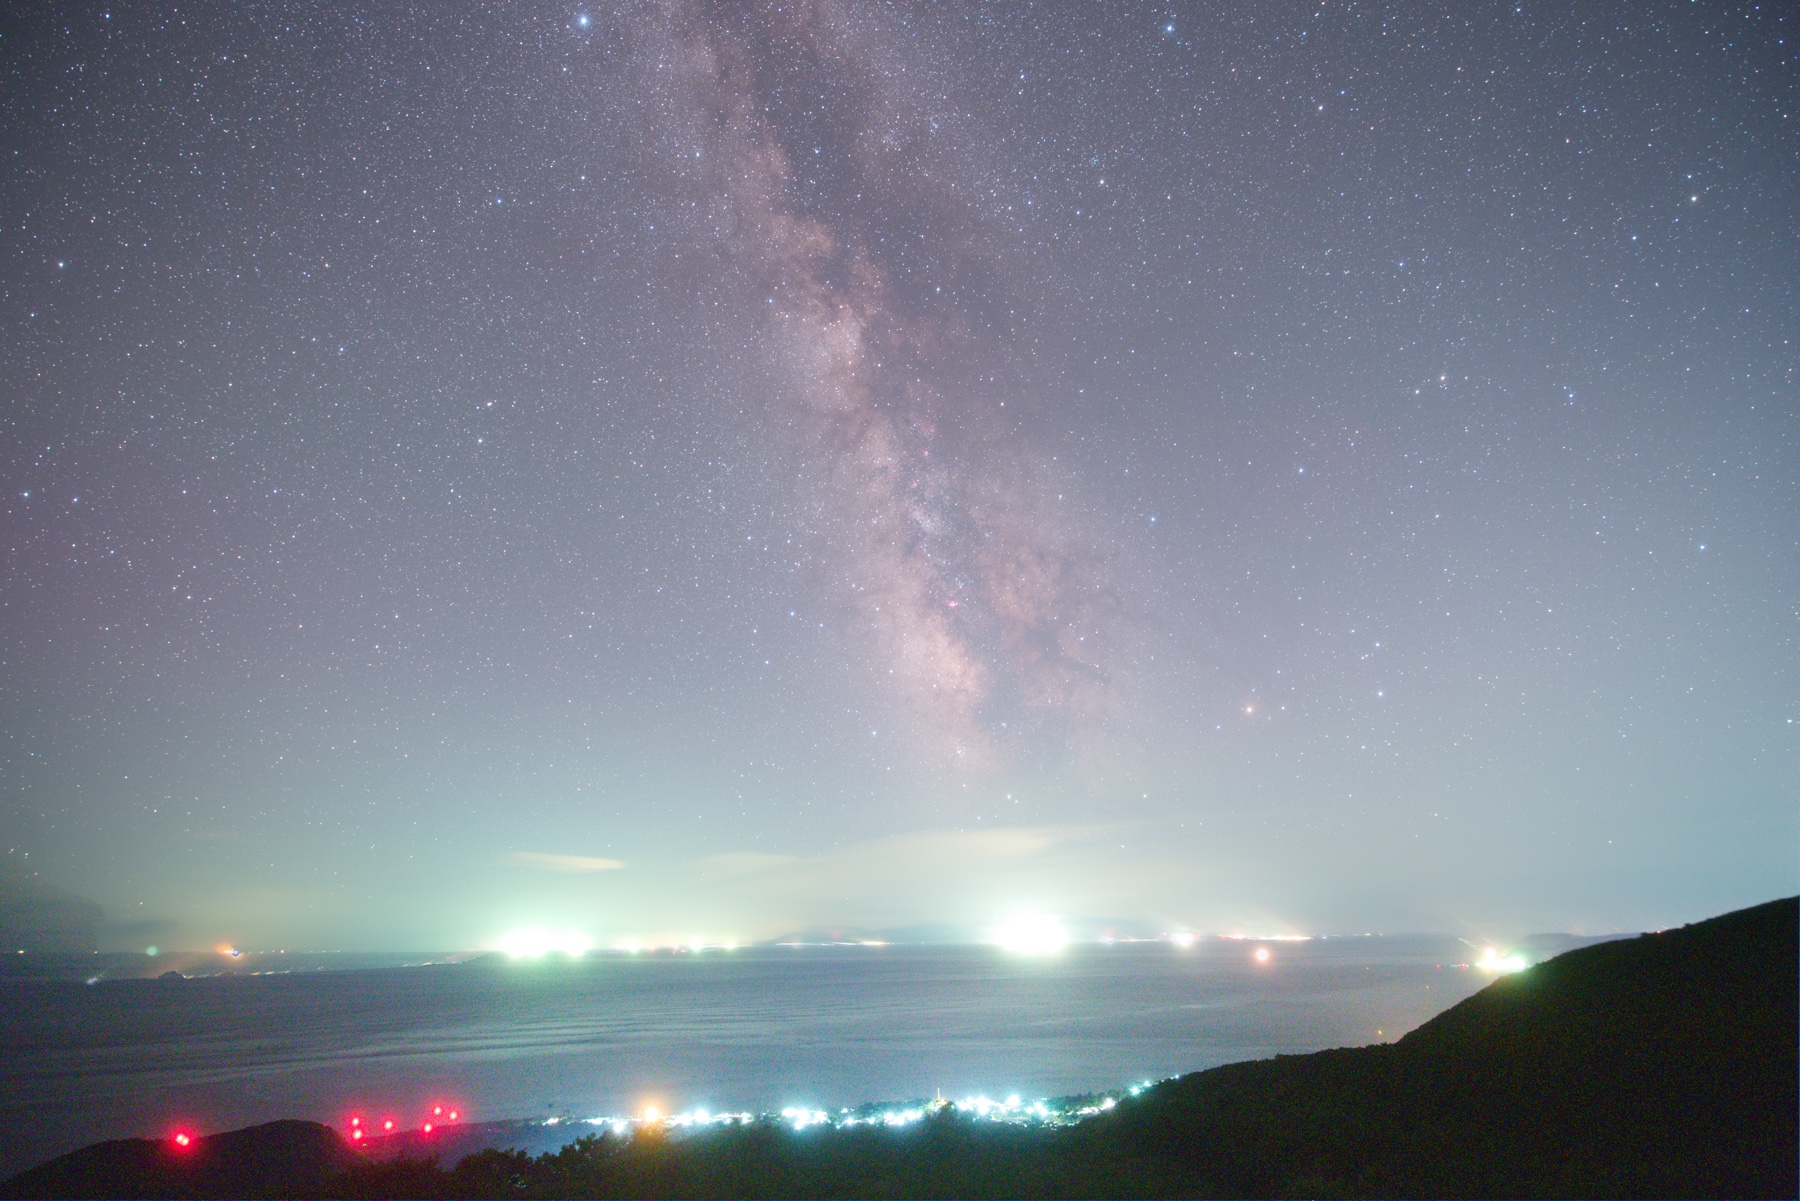
\includegraphics[width=\linewidth]{figures/photo_groundfixed}
\caption{地上固定フレーム（2枚、露出の違う AEB）を使って合成した例}
\end{figure}

\subsection{境界ぼかし}\label{sec:feather}

\ui{境界ぼかし}（0〜300 px）を大きくすると、空と地上の境目をなだらかにつなぎます。最初は 0 px（自動で決めた境目のまま）です。
\begin{itemize}[itemsep=0.3ex]
  \item 境目に線のような段差が見えるときに使います。100〜200 px くらいから試してください。
  \item 地上固定フレームを使うときは、地上の側にだけぼかします。空の星はそのままで、地上固定フレームのノイズや色味の違いを、境目の近くでなだらかにつなぎます。
  \item プレビューのマスクも、合成と同じだけぼかして表示されます。
\end{itemize}

\subsection{うまくいかないとき}

\begin{center}
\small
\begin{tabularx}{\linewidth}{>{\raggedright\arraybackslash}p{0.38\linewidth} X}
\toprule
表示・ようす & どうすればよいか \\
\midrule
「星と地上の動きの差が小さいため、空と地上を分けずに合成しました」 & 撮影時間が短く、星がほとんど動いていません。ふつうの合成で十分きれいになります。 \\
「空と地上をはっきり見分けられなかったため…」 & 空だけ・地上だけの構図です。ブラシで空と地上を塗ってから、もう一度\ui{解析開始}を押してみてください。 \\
空の一部が地上（または地上の一部が空）になる & ブラシで塗り直してから、スタッキング開始を押します。 \\
地上の明るい灯りのまわりが不自然 & 灯りのまわりを空（青）か地上（緑）で塗り分けると、改善することがあります。 \\
「…のメモリが必要なため実行できません」 & 写真の枚数を減らしてください。 \\
\bottomrule
\end{tabularx}
\end{center}
